\chapter{Wprowadzenie}
\large{
Badanie elektrokardiograficzne, dzięki swej dostępności i łatwości wykonania stanowi jedno z najczęściej wykorzystywanych metod rozpoznawania zaburzeń w pracy serca. Uzyskiwany przy jego pomocy sygnał EKG dostarcza informacji o elektrycznej aktywności mięśnia sercowego, jako różnicę potencjałów pomiędzy dwoma elektrodami.

Jednym z najbardziej charakterystycznych elementów typowego sygnału EKG są zespoły QRS. Jest to układ trzech załamków opisujących proces depolaryzacji mięśnia. Ideowy schemat EKG, wraz z kompleksem QRS przedstawiono na rysunku \ref{fig:qrs-complex}.


\begin{figure}[H]
	\centering
	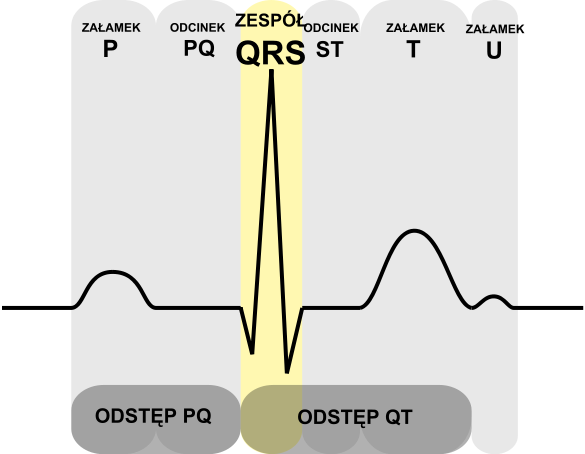
\includegraphics[width=8cm]{img/qrs-complex}
	\caption{Ideowy schemat sygnału EKG. Źródło: \cite{qrs-wiki}}
	\label{fig:qrs-complex}
\end{figure}

Na podstawie kształtu zespołu QRS diagnozować można szereg dysfunkcji serca. Wykorzystanie w tym celu zautomatyzowanych procedur diagnostycznych pozwala na zwiększenie prawdopodobieństwa wykrycia nieprawidłowości i przyśpiesza proces badania.

Klasyfikacja zespołów QRS pozwala na wyodrębnienie grup kompleksów o podobnych parametrach. Wykorzystać w tym celu można bazę \textit{MIT-DB} \cite{mitdb}, zawierającą kilkadziesiąt sygnałów referencyjnych, wraz z precyzyjnym opisem stanu pacjenta i wykrytych nieprawidłowości.
}
